\documentclass{beamer}
\usetheme{metropolis}

\usetheme{metropolis}

\usepackage[ngerman]{babel}
\usepackage[autostyle=true,german=quotes]{csquotes}
\usepackage[linewidth=1pt]{mdframed}
\usepackage{hyperref}
\usepackage{makecell}
\usepackage{pifont}
\usepackage{tikz}
\usetikzlibrary{positioning, calc, arrows, fit, decorations.pathreplacing, shapes, shapes.multipart, snakes}
\usepackage{verbatim}
\usepackage{textcomp}
\usepackage{centernot}
\usepackage{tabularx}
\usepackage{ulem}
%\usepackage{pdfpages}

\batchmode

\hypersetup{
	colorlinks,
	urlcolor=blue,
	linkcolor=black % for ToC
}
\newenvironment{qaa}[1]{
	#1

	\begin{mdframed}
		\small
}{
	\end{mdframed}
}

\newcommand{\true}{\ding{51}}
\newcommand{\false}{\ding{55}}
\newcommand{\code}[1]{
	\begin{mdframed}
		\verbatiminput{#1}
	\end{mdframed}
}


\title{Tutorium 04: $\lambda$-Kalkül}
% \subtitle{}
\author{David Kaufmann}
\institute{Tutorium Programmierparadigmen am KIT}
\date{23. November 2022}

\begin{document}

\begin{frame}
	\titlepage
\end{frame}

\section{Übungsblatt 3}

\begin{frame}{1 --- Streams}
    \only<1>{
        \code{../demos/Fibs.hs}

        Auswertung:

        \code{code/Fibs.eval}
    }
    \only<2>{
        \begin{center}
            \texttt{fibs = 0 : (1 : zipWith (+) fibs (tail fibs))}
        \end{center}
        \begin{columns}
            \begin{column}{0.6\textwidth}
                \begin{figure}
                    \begin{tikzpicture}[node font=\ttfamily, level distance=0.8cm, sibling distance=1.2cm, every node/.style={scale=0.8}]
                        \node (def) {fibs};
                        \node[below=0.8cm of def] (root) {(:)}
                            child {
                                node {0}
                            }
                            child {
                                node {(:)}
                                child {
                                    node {1}
                                }
                                child {
                                    node {zwp}
                                    child {
                                        node (u1) {$\to$}
                                    }
                                    child {
                                        node {tail}
                                        child {
                                            node (u2) {$\to$}
                                        }
                                    }
                                }
                            }
                        ;
                        \draw[->] (def) -- (root);
                        \draw[->] (u1) edge [bend left=120] (root);
                        \draw[->] (u2) edge [bend right=80] (root);
                    \end{tikzpicture}
                \end{figure}
            \end{column}
            \begin{column}{0.4\textwidth}
                \footnotesize
                \begin{itemize}
                    \item \texttt{zwp = zipWith (+)}
                    \item Laufzeit: Alle Vorkommen von \texttt{fibs} beziehen sich auf dasselbe Speicherobjekt (Sharing)
                    \pause
                    \item \texttt{tail (x:xs) = xs}
                \end{itemize}
            \end{column}
        \end{columns}
    }
    \only<3>{
        \begin{columns}
            \begin{column}{0.6\textwidth}
                \begin{figure}
                    \begin{tikzpicture}[node font=\ttfamily, level distance=0.8cm, sibling distance=1.2cm, every node/.style={scale=0.8}]
                        \node (def) {fibs};
                        \node[below=0.8cm of def] (root) {(:)}
                            child {
                                node {0}
                            }
                            child {
                                node (second) {(:)}
                                child {
                                    node[draw] {1}
                                }
                                child {
                                    node {zwp}
                                    child {
                                        node (u1) {$\to$}
                                    }
                                    child {
                                        node (u2) {$\to$}
                                    }
                                }
                            }
                        ;
                        \draw[->] (def) -- (root);
                        \draw[->] (u1) edge [bend left=120] (root);
                        \draw[->] (u2) edge [bend right=80] (second);
                    \end{tikzpicture}
                \end{figure}
            \end{column}
            \begin{column}{0.4\textwidth}
                \footnotesize
                \begin{itemize}
                    \item \texttt{tail (x:xs) = xs}
                    \item \texttt{fibs !! 1 == 1}
                    \item Keine Berechnung notwendig
                    \item \texttt{fibs !! 3}?
                \end{itemize}
            \end{column}
        \end{columns}
    }
    \only<4>{
        \begin{columns}
            \begin{column}{0.6\textwidth}
                \begin{figure}
                    \begin{tikzpicture}[node font=\ttfamily, level distance=0.8cm, sibling distance=1.2cm, every node/.style={scale=0.8}]
                        \node (def) {fibs};
                        \node[below=0.8cm of def] (root) {(:)}
                            child {
                                node {0}
                            }
                            child {
                                node (second) {(:)}
                                child {
                                    node {1}
                                }
                                child {
                                    node (third) {(:)}
                                    child {
                                        node[draw] {1}
                                    }
                                    child {
                                        node {zwp}
                                        child {
                                            node (u1) {$\to$}
                                        }
                                        child {
                                            node (u2) {$\to$}
                                        }
                                    }
                                }
                            }
                        ;
                        \draw[->] (def) -- (root);
                        \draw[->] (u1) edge [bend left=120] (second);
                        \draw[->] (u2) edge [bend right=80] (third);
                    \end{tikzpicture}
                \end{figure}
            \end{column}
            \begin{column}{0.4\textwidth}
                \footnotesize
                \begin{itemize}
                    \item \texttt{zwp (x:xs) (y:ys) = (x + y) : zwp xs ys}
                    \item \texttt{fibs !! 2 == 1}
                    \item \texttt{fibs !! 3}?
                \end{itemize}
            \end{column}
        \end{columns}
    }
    \only<5>{
        \begin{columns}
            \begin{column}{0.6\textwidth}
                \begin{figure}
                    \begin{tikzpicture}[node font=\ttfamily, level distance=0.8cm, sibling distance=1.2cm, every node/.style={scale=0.8}]
                        \node (def) {fibs};
                        \node[below=0.8cm of def] (root) {(:)}
                            child {
                                node {0}
                            }
                            child {
                                node (second) {(:)}
                                child {
                                    node {1}
                                }
                                child {
                                    node (third) {(:)}
                                    child {
                                        node {1}
                                    }
                                    child {
                                        node (fourth) {(:)}
                                        child {
                                            node[draw] {2}
                                        }
                                        child {
                                            node {zwp}
                                            child {
                                                node (u1) {$\to$}
                                            }
                                            child {
                                                node (u2) {$\to$}
                                            }
                                        }
                                    }
                                }
                            }
                        ;
                        \draw[->] (def) -- (root);
                        \draw[->] (u1) edge [bend left=120] (third);
                        \draw[->] (u2) edge [bend right=80] (fourth);
                    \end{tikzpicture}
                \end{figure}
            \end{column}
            \begin{column}{0.4\textwidth}
                \footnotesize
                \begin{itemize}
                    \item \texttt{zwp (x:xs) (y:ys) = (x + y) : zwp xs ys}
                    \item \texttt{fibs !! 3 == 2}
                    \item \texttt{zwp} verschiebt nur Zeiger auf bestehendes Objekt, \texttt{fibs} wird nur einmal berechnet und steht ab da zur Verfügung
                \end{itemize}
            \end{column}
        \end{columns}
    }
\end{frame}

\begin{frame}{\texttt{:sprint}}
	\code{code/ghci-sprint.output}

	\begin{itemize}
		\item \texttt{:sprint a} gibt aktuelle Speicherrepräsentation für \texttt{a} aus
		\item \texttt{\_} steht dabei für \enquote{noch nicht ausgewertet}
		\item $\leadsto$ praktisch für Debugging unendlicher Listen
	\end{itemize}
\end{frame}

\begin{frame}{Prime Powers}
    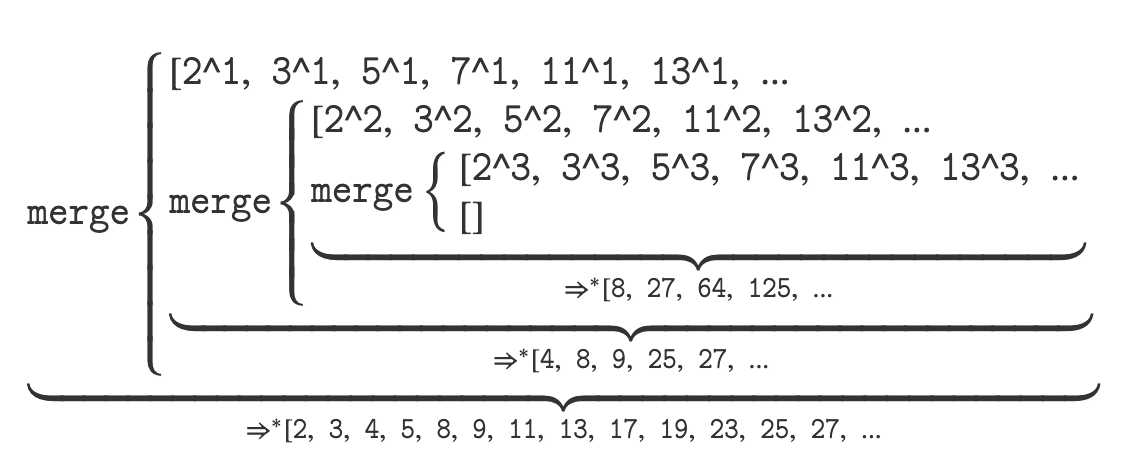
\includegraphics[scale=0.27]{slides/images/primepowers.png}
\end{frame}

\section{Wiederholung: Algebraische Datentypen}

\begin{frame}{Cheatsheet: Algebraische Datentypen in Haskell}
  \begin{itemize}
    \item \emph{\texttt{data}-Definitionen}, \emph{Datenkonstruktoren}
    \item Algebraische Datentypen: \emph{Produkttypen} und \emph{Summentypen}
    \begin{itemize}
      \item Produkttypen $\approx$ \texttt{struct}s in C
      \item Summentypen $\approx$ \texttt{enum}s
    \end{itemize}
    \item \emph{Typkonstruktoren}, bspw. \texttt{[] :: * -> *}
    \item \emph{Polymorphe} Datentypen, bspw. \texttt{[a]}, \texttt{Maybe a}
    \item Beispiel:
  \end{itemize}
  \code{../demos/Shape.hs}
\end{frame}

\begin{frame}{Cheatsheet: Typklassen 1}
  \begin{itemize}
    \item \emph{Klasse}, \emph{Operationen}/\emph{Methoden}, \emph{Instanzen}
    \item Beispiele:
    \begin{itemize}
      \item \texttt{Eq t}, $\{ \texttt{(==)}, \texttt{(/=)} \}$, $\{ \texttt{Eq Bool}, \texttt{Eq Int}, \texttt{Eq Char}, ... \}$
      \item \texttt{Show t}, $\{ \texttt{show} \}$, $\{ \texttt{Show Bool}, \texttt{Show Int}, \texttt{Show Char}, ... \}$
    \end{itemize}
    \item Weitere Typklassen: \texttt{Ord}, \texttt{Num}, \texttt{Enum}
    \item Deklaration/Implementierung:
  \end{itemize}

  \code{../demos/Truthy.hs}
\end{frame}

\begin{frame}{Cheatsheet: Typklassen 2}
  \begin{itemize}
    \item \emph{Vererbung}: Typklassen mit Voraussetzungen
  \end{itemize}

  \code{../demos/Truthy2.hs}
\end{frame}

\begin{frame}{Spielkarten}
  \code{../demos/PlayingCard.hs}
\end{frame}

\begin{frame}{Boolesche Logik}
  \code{../demos/BoolExpr.hs}

  \vfill

  Beispiele:
  \begin{itemize}
    \item $a \wedge b$ entspricht \texttt{BinaryOp (Var "{}a"{}) AND (Var "{}b"{})}
    \item $a \vee (b \wedge 0)$ entspricht\\
          \texttt{BinaryOp (Var "{}a"{}) AND (BinaryOp (Var "{}b"{}) OR (Const False))}
  \end{itemize}
\end{frame}

\section{$\lambda$-Kalkül}

\begin{frame}{$\lambda$-Kalkül}
	\begin{itemize}
                \item \enquote{Funktionales Gegenstück zur Turingmaschine}
		\item Gönnt Punkte in der Klausur
	\end{itemize}
\end{frame}

\begin{frame}{$\lambda$-Terme}
	Ein Term im $\lambda$-Kalkül hat eine der drei folgenden Formen:

	\vspace{0.5cm}

	\begin{tabularx}{\textwidth}{ X | X | X }
		\textbf{Notation} & \textbf{Besteht aus}                      & \textbf{Bezeichnung} \\
		\hline
		$x$               & $x$ : Variablenname                       & Variable             \\
		\hline
		$\lambda{}p.b$    &
			\begin{tabular}[t]{@{}c@{}}$p$ : Variablenname\\$b$ : $\lambda$-Term\end{tabular}
									      & Abstraktion          \\
		\hline
		$f$ $a$           & $f$, $a$ : $\lambda$-Terme                & Funktionsanwendung   \\
	\end{tabularx}

	\vspace{0.5cm}

	\begin{itemize}
		\item \enquote{$\lambda$-Term}: rekursive Datenstruktur
		\item Semantik definieren wir später
		\pause
		\item Jetzt: Ergänzt das Modul \texttt{Lambda} um die fehlenden Typen
		\begin{itemize}
			\item +Fragen zur ÜB-Korrektur
		\end{itemize}
	\end{itemize}
\end{frame}

\begin{frame}{$\lambda$-Terme in Haskell}
	\code{../demos/Lambda.hs}

    \begin{itemize}
        \item Variable $x$ hat einen Variablennamen $x$
        \item Funktionsanwendung $\app{f}{a}$ hat zwei $\lambda$-Terme: Funktion $f$ und Argument $a$
        \item Abstraktion $\lam{p}{b}$ hat Variablennamen $p$ als Parameter und $\lambda$-Term $b$ als Körper (Body)
    \end{itemize}
\end{frame}

\newcommand{\aeq}{\stackrel{\alpha}{=}}
\newcommand{\naeq}{\stackrel{\alpha}{\neq}}
\newcommand{\eeq}{\stackrel{\eta}{=}}

\newcolumntype{s}{>{\hsize=.8\hsize}X}

\begin{frame}{Begriffe im $\lambda$-Kalkül}
	\fontsize{9pt}{13}\selectfont

	\begin{tabularx}{\textwidth}{ s | X | X }
		\textbf{Begriff} & \textbf{Formel} & \textbf{Bedeutung} \\
		\hline
		$\alpha$-Äquivalenz & $t_1 \aeq t_2$ & $t_1$, $t_2$ sind gleicher Struktur \\
		\hline
		$\eta$-Äquivalenz & $\lambda{}x.f$ $x \eeq f$ & \enquote{Unterversorgung} \\
		\hline
		Freie Variablen & $fv(\lambda{}p.b) = { b }$ & Menge der nicht durch $\lambda$s gebundenen Variablen \\
		\hline
		Substitution & $(\lambda{}p.b)\left[b\rightarrow{}c\right]=\lambda{}p.c$ & Ersetzung freier Variablen \\
		\hline
		Redex & $(\lambda{}p.b)$ $t$ & \enquote{Reducible expression} \\
		\hline
		$\beta$-Reduktion & $(\lambda{}p.b)$ $t \Rightarrow b\left[p\rightarrow{}t\right]$ & \enquote{Funktionsanwendung} \\
	\end{tabularx}
\end{frame}

\subsection{Substitution, Freie Variablen}

\begin{frame}{Freie Variablen}
	\begin{itemize}
		\item $fv(t)$ bezeichnet die frei vorkommenden Variablen im Term $t$
		\item Frei vorkommend $\approx$ nicht durch ein $\lambda$ gebunden
		\begin{itemize}
			\item $fv(x) = \{x\}$, wenn $x$ Variable
			\item $fv(f$ $x) = fv(f) \cup fv(x)$
			\item $fv(\lambda{}p.b) = fv(b) \setminus \{p\}$
		\end{itemize}
		\item Beispiele:
		\begin{itemize}
			\item $fv(\lambda{}x.x) = \emptyset$
			\item $fv(\lambda{}x.y) = \{y\}$
		\end{itemize}
		\pause
		\item Implementiert \texttt{fv :: LambdaTerm -> Set String}
		\begin{itemize}
			\item Benutzt \texttt{Set}, \texttt{union}, \texttt{delete} und \texttt{fromList} aus \texttt{Data.Set}
            \item Bspw. \texttt{fv (Abs "p" (Var "b")) == fromList ["b"]}
		\end{itemize}
	\end{itemize}
\end{frame}

\begin{frame}{Substitution}
	\begin{itemize}
		\item Substitution ersetzt alle \emph{freien} Variablen in einem Term
		\item $t\left[a \to b\right]$ --- Ersetze $a$ durch $b$ in $t$
		\item Beispiele:
		\begin{itemize}
			\item $a\left[a \to b\right] = b$
			\item $a\left[b \to c\right] = a$
			\item $(f$ $x)\left[f \to g\right]\left[x \to y\right] = g$ $y$
			\pause
			\item $(\lambda{}x.f$ $x)\left[x \to y\right] = \lambda{}x.f$ $x$ ($x$ ist nicht frei)
			\item $(\lambda{}x.f$ $x)\left[f \to g\right] = \lambda{}x.g$ $x$ ($f$ ist frei)
		\end{itemize}
		\pause
		\item Implementiert\\
		      \texttt{substitute :: (String, Term) -> Term -> Term}
		\begin{itemize}
			\item \texttt{type Term = LambdaTerm}
			\item Tipp: Dafür braucht ihr \texttt{fv}
		\end{itemize}
	\end{itemize}
\end{frame}

\subsection{Äquivalenz}

\begin{frame}{$\alpha$-Äquivalenz}
	\begin{itemize}
		\item $t_1 \aeq t_2$ --- Strukturelle Äquivalenz der Terme $t_1$ und $t_2$
		\item Umformung von $t_1$ in $t_2$ allein durch Substitution der (gebundenen) Variablen möglich
		\pause
		\item Bspw.:
		\begin{itemize}
			\item $x \naeq y$, da $x$ und $y$ frei sind
			\item $\lambda{}x.x \aeq \lambda{}y.y$, durch Umbenennen von $x$ zu $y$
			\item $f$ $(\lambda{}x.y) \aeq f$ $(\lambda{}p.y)$
			\item $\lambda{}x.y \naeq \lambda{}x.z$
		\end{itemize}
	\end{itemize}
\end{frame}

\begin{frame}{$\eta$-Äquivalenz}
	\begin{itemize}
		\item $\lambda{}x.f$ $x \eeq f$, wenn $x \notin fv(f)$
		\item Wie bei Haskell:\\
	              \texttt{all list = foldl (\&\&) True list} $\Leftrightarrow$\\
		      \texttt{all = \textbackslash{}list -> foldl (\&\&) True list} $\Leftrightarrow$\\
		      \texttt{all = foldl (\&\&) True}
		\item Also:
		\begin{itemize}
			\item $\eta$-Äquivalenz: eher Umformungsschritt als Gleichheitskriterium
			\item Formelle Definition von Unterversorgung
		\end{itemize}
	\end{itemize}
\end{frame}

\subsection{Redex, $\beta$-Reduktion}

\begin{frame}{$\beta$-Reduktion}
	\begin{itemize}
		\item Bisher: $\lambda$-Terme als (seltsame) Datenstruktur\\
		      Jetzt: Ausführungssemantik
		\pause
		\item RedEx: \enquote{Reducible expression} $\Leftrightarrow$\\
		      Funktionsanwendung ($f$ $a$), mit $f = \lambda{}p.b$
	      \item $(\lambda{}p.b)$ $a\pause \implies b\left[p \to a\right]$
		\pause
		\item \enquote{Ausführung} (besser: Auswertung) von $\lambda$-Termen: Anwenden der $\beta$-Reduktion, bis Term \enquote{konvergiert}
		\item Term konvergiert $\approx$ Normalform $\approx$ enthält keinen Redex mehr
		\begin{itemize}
			\item Notation: $t \centernot\implies$
		\end{itemize}
		\pause
		\item $id$ $a = (\lambda{}x.x)$ $a \implies x\left[x \to a\right] = a \centernot\implies$
	\end{itemize}
\end{frame}

\begin{frame}{Beispiel: Church-Booleans}
  \begin{eqnarray*}
    \ctrue &= \lam{x}{\lam{y}{x}} \\
    \cfalse &= \lam{x}{\lam{y}{y}} \\
    \cand &= \lam{a}{\lam{b}{\app{\app{a}{b}}{\cfalse}}} \\
          &= \lam{a}{\lam{b}{\app{(\app{a}{b})}{\cfalse}}} \\
  \end{eqnarray*}

  Funktioniert $\cand$? $\leadsto$ Wahrheitstabelle aufstellen:

  \begin{eqnarray*}
    &\app{\app{\cand}{\ctrue}}{\ctrue} = \app{\app{(\uline{\lam{a}{\lam{b}{\app{\app{a}{b}}{\cfalse}}}})}{\ctrue}}{\ctrue} \\
    \pause
    &\Rightarrow_\beta \app{(\lam{b}{\app{\app{a}{b}}{\cfalse}})\left[ a \to \ctrue \right]}{\ctrue} = \app{(\uline{\lam{b}{\app{\app{\ctrue}{b}}{\cfalse}}})}{\ctrue} \\
    \pause
    &\Rightarrow_\beta (\app{\app{\ctrue}{b}}{\cfalse}) \left[ b \to \ctrue \right] = \app{\app{(\uline{\lam{x}{\lam{y}{x}}})}{\ctrue}}{\cfalse} \\
    \pause
    &\Rightarrow_\beta \app{(\uline{\lam{y}{\ctrue}})}{\ctrue} \Rightarrow_\beta \ctrue \;\; \text{\true}
  \end{eqnarray*}
\end{frame}

\begin{frame}{Beispiel: Church-Booleans}
  \begin{eqnarray*}
    &\app{\app{\cand}{\cfalse}}{t} = \app{\app{(\uline{\lam{a}{\lam{b}{\app{\app{a}{b}}{\cfalse}}}})}{\cfalse}}{t} \\
    \pause
    &\Rightarrow_\beta \app{(\lam{b}{\app{\app{a}{b}}{\cfalse}})\left[ a \to \cfalse \right]}{t} = \app{(\uline{\lam{b}{\app{\app{\cfalse}{b}}{\cfalse}}})}{t} \\
    \pause
    &\Rightarrow_\beta (\app{\app{\ctrue}{b}}{\cfalse}) \left[ b \to t \right] = \app{\app{(\uline{\lam{x}{\lam{y}{y}}})}{t}}{\cfalse} \\
    \pause
    &\Rightarrow^2 \cfalse
  \end{eqnarray*}

  \begin{eqnarray*}
    &\app{\app{\cand}{t}}{\cfalse} = \app{\app{(\uline{\lam{a}{\lam{b}{\app{\app{a}{b}}{\cfalse}}}})}{t}}{\cfalse} \\
    \pause
    &\Rightarrow_\beta \app{(\lam{b}{\app{\app{a}{b}}{\cfalse}})\left[ a \to t \right]}{\cfalse} = \app{(\uline{\lam{b}{\app{\app{t}{b}}{\cfalse}}})}{\cfalse} \\
    \pause
    &\Rightarrow_\beta (\app{\app{t}{b}}{\cfalse}) \left[ b \to \cfalse \right] = \app{\app{t}{\cfalse}}{\cfalse} \\
    \pause
    &\leadsto \cfalse
  \end{eqnarray*}
\end{frame}

\end{document}
